
% --------------------------------------------------------------- CONFIGURATIONS

\documentclass[a4paper,12pt,final,oneside]{book}

\usepackage{rapport}


% -------------------------------------------------------------- META: CONSTANTS

\newcommand{\reporttitle}{Grammaire et langage}
\newcommand{\enseignants}{Nabila~\textsc{Benharkat}\\Eric~\textsc{Guérin}}
\newcommand{\reportauthor}{Guillaume~\textsc{Abadie}\\Thierry~\textsc{Cantenot}\\Juliette~\textsc{Courlet}\\Rémi~\textsc{Domingues}\\Adrien~\textsc{Duffy-Coissard}\\Ahmed~\textsc{Kachkach}}
\newcommand{\reportsubject}{Livrable de projet}
\newcommand{\stagetopic}{Analyse de fichiers XML}
\newcommand{\dateperiod}{du 14 Mars au XX Mars 2014}
\newcommand{\HRule}{\rule{\linewidth}{0.5mm}}
\setlength{\parskip}{1ex} % Espace entre les paragraphes

\hypersetup{
	pdftitle={\reporttitle},%
		pdfauthor={\reportauthor},%
		pdfsubject={\reportsubject},%
		pdfkeywords={INSA Lyon} {Grammaire et langage}
}

\title{\reporttitle}
\author{\reportauthor}
%\setcounter{tocdepth}{4}


% ------------------------------------------------------------------------- FILE

\begin{document}


    % ------------------------------------------------------------------- HEADER

	\renewcommand{\chaptername}{} %\renewcommand{\thechapter}{}
	\renewcommand{\contentsname}{Sommaire}

	\pagestyle{empty}
	\pagenumbering{Roman}


    % ------------------------------------------------------------ HEADER: TITLE

	% Inspiré de http://en.wikibooks.org/wiki/LaTeX/Title_Creation
\begin{center}
	\begin{minipage}[t]{0.48\textwidth}
	  \begin{flushleft}
	    
\includegraphics [width=40mm]{images/logo_INSA.png} \\[0.5cm]
			INSA Lyon\\
			20, avenue Albert Einstein\\
			69621 Villeurbanne Cedex
	  \end{flushleft}
	\end{minipage}
	\begin{minipage}[t]{0.48\textwidth}
	  \begin{flushright}
	    %\includegraphics [width=60mm]{images/logo_Passau.jpg} \\[0.5cm]
	    %Universität Passau\\
		%Innstraße, 3\\
		%	D-94032 Passau
	  \end{flushright}
	\end{minipage} \\[2cm]

	\textsc{\Large \reportsubject}\\[0.3cm]
	\HRule \\[0.4cm]
	{\Huge \bfseries \reporttitle}\\[0.3cm]
	{\LARGE \bfseries «~\stagetopic~»}\\[0.3cm]
	{\Large \dateperiod}\\[0.4cm]
	\HRule \\[1cm]

	
\includegraphics [scale=0.35]{images/application-xml.png} \\[0.7cm]
	\begin{minipage}[t]{0.4\textwidth}
	  \begin{flushleft} \large
	    \emph{Hexanôme~:}\\
	    \small \reportauthor
	  \end{flushleft}
	\end{minipage}
	\begin{minipage}[t]{0.5\textwidth}
	  \begin{flushright} \large
	    \emph{Enseignants~:} \\
	    \enseignants
	  \end{flushright}
	\end{minipage}

	\vfill
	\footnotesize{Année scolaire 2013-2014}
\end{center}



    % --------------------------------------------------- HEADER: CONFIGURATIONS

	\sloppy          % Justification moins stricte : des mots ne dépasseront pas des paragraphes

    \frontmatter
		\pagestyle{empty}
		\tableofcontents
		\addtocontents{toc}{\protect\thispagestyle{empty}}

	\mainmatter
	\pagestyle{headings}

	\renewcommand{\chaptermark}[1]{\markboth{\MakeUppercase{\chaptername\ \thechapter.\ #1}}{}}
	\renewcommand{\sectionmark}[1]{\markright{\thesection{} #1}}


    % ------------------------------------------------------------------ CONTENT

	\chapter{Chapitre trololo}

Trololo et tralala.

	\chapter{Diagramme de classes}
Les documents XML bien formés répondront à l'arborescence présentée ci-dessous.

Les hypothèse suivantes sont également formulées :
\begin{itemize}
    \item Les documents XML à parser ne contiendront pas de DTD interne
    \item Les Process Instruction (PI) ne contiendront que des attributs
    \item Aucune référence ne sera présente dans les documents XML\\
\end{itemize}

Les classes ici décrites seront rattachées au namespace XML défini en C++.

\begin{itemize}
    \addtolength{\itemindent}{10px}
    \item \textbf{Document} : Cette classe contient un prolog, un élément racine de type Element et un ensemble de fils de type DocumentNode (liste pouvant contenir 0 à N éléments).
    \item \textbf{MiscNode} : Cette classe abstraite permet à la classe Document de contenir 0 à N éléments Misc.
    On notera ici qu'une relation de spécialisation représente le symbole $'|'$ (alternative) dans une règle BNF.
    \item \textbf{Comment} : Contient la description d'un commentaire sous forme de chaîne de caractères.
    \item \textbf{Processing Instruction} : En accord avec l'hypothèse énoncée précédemment, une PI ne contient qu'un nom et une liste ordonnée d'attributs
    \item \textbf{Attribute} : Cette classe décrit un attribut sous la forme suivante : mName = "mValue"
    \item \textbf{DocumentNode} : Une instance de cette classe peut être de type Element, Text Comment ou PI. Afin de garantir la cohérence de l'architecture XML, ce noeud dispose d'un pointeur sur son noeud parent.
    \item \textbf{Element} : Un élément XML dispose d'un nom de balise, d'un ensemble ordonné d'attributs et d'un ensemble ordonné de noeuds fils. Cet élément peut être une balise vide ($<br/>$).
    \item \textbf{Text} : Un noeud texte est naturellement décrit par une chaîne de caractères.
    \item \textbf{ElementIterator} : Cet élément est dédié au parcours de l'arbre XML, de manière similaire à un parseur de type SAX.
\end{itemize}

\begin{landscape}
\begin{figure}[h!]
    \centering
    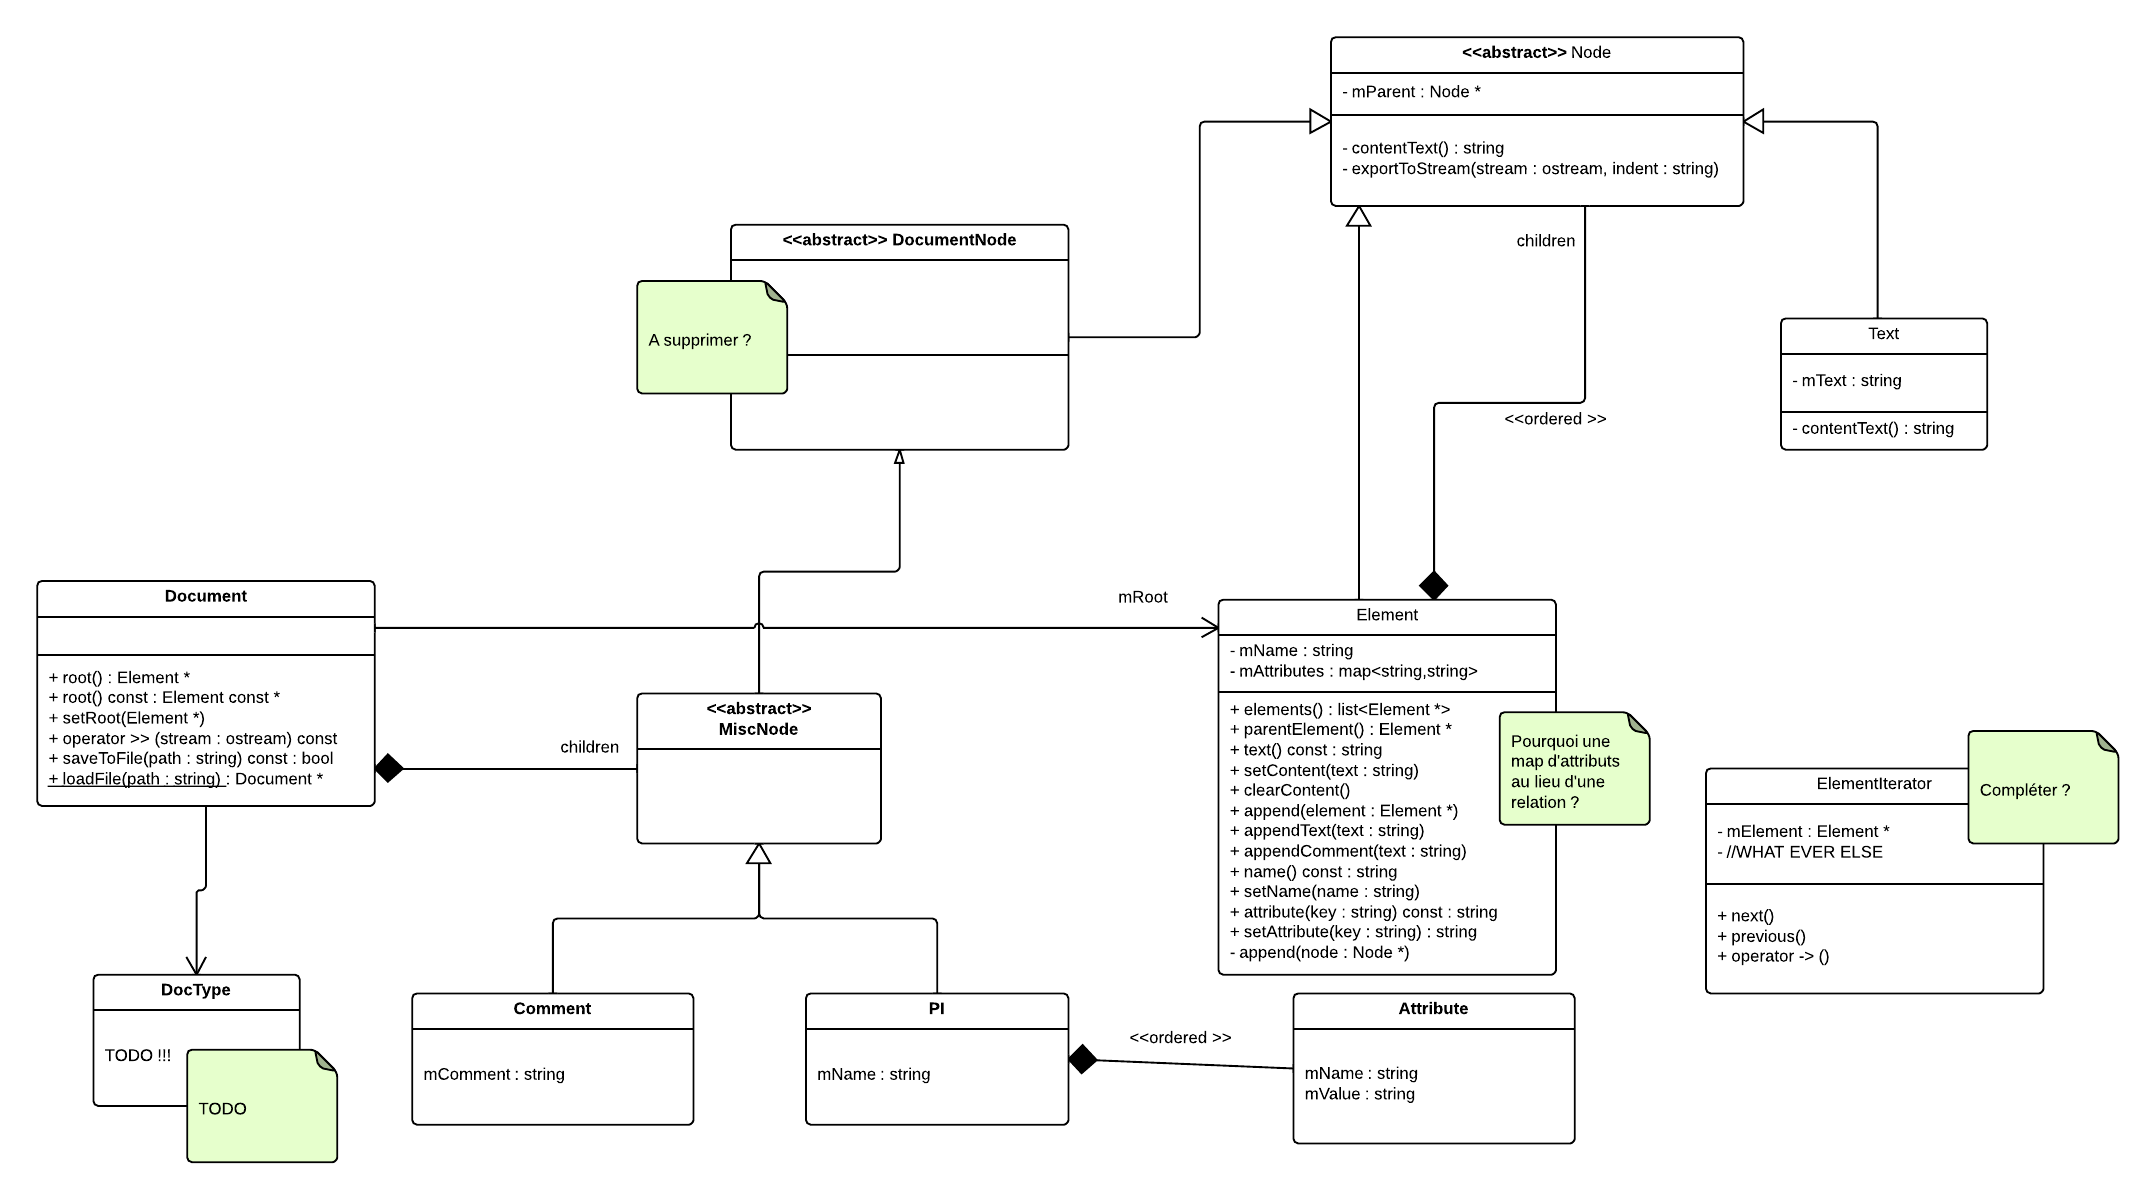
\includegraphics[width=\linewidth]{images/classDiagram.png}
    \caption{Diagramme de classes de l'arborescence XML}
    \label{classDiagram}
\end{figure}
\end{landscape}


	%\renewcommand{\chaptermark}[1]{\markboth{\MakeUppercase{#1}}{}}
	%\renewcommand{\sectionmark}[1]{\markright{#1}}

	%\addcontentsline{toc}{part}{Annexes}
	%\part*{Annexes}
	%\appendix
	%\include{implementationExercices}


    % ------------------------------------------------------------------- FOOTER
\end{document}
